\section{Alternative Concept: The Universal Removable Battery Standard}
\label{sec:alternative}

Based on the LCA results identifying \todo{specify greatest impact --- likely battery materials and end-of-life landfilling} as the dominant environmental impact, this section presents an alternative concept designed to minimize these impacts: a \textbf{universal removable battery standard} for electronic cigarettes.

\subsection{Design Rationale}

The Oxford/UCL study demonstrated that lithium-ion cells in disposable e-cigarettes can sustain over 450 charge--discharge cycles \cite{williams2023}, yet are discarded after a single use. The core insight driving this concept is that the battery---the most environmentally impactful component---can be \textbf{decoupled from the consumable portion} of the device and \textbf{standardized across manufacturers}.

This approach draws on precedent from:
\begin{itemize}
    \item The AA/AAA battery standard (IEC 60086), which enables interchangeability across thousands of products from hundreds of manufacturers
    \item The EU Batteries Regulation (Article 11), which mandates removable, replaceable batteries in portable electronics by February 2027 \cite{eu_batteries_2023}
    \item The Fairphone modular smartphone design, which demonstrates commercial viability of DfD consumer electronics
\end{itemize}

\subsection{Proposed Standard Specification}

The standard defines \textbf{three battery form factors} covering the full range of disposable e-cigarette capacities:

\begin{table}[H]
\centering
\caption{Proposed universal e-cigarette battery standard --- three sizes.}
\label{tab:battery_standard}
\begin{tabular}{@{}lcccl@{}}
\toprule
\textbf{Size Class} & \textbf{Diameter (mm)} & \textbf{Length (mm)} & \textbf{Capacity (mAh)} & \textbf{Use Case} \\
\midrule
VC-S (Small)   & \todo{8--10}  & \todo{30--35} & 280--400  & Compact / low-puff devices \\
VC-M (Medium)  & \todo{10--13} & \todo{35--45} & 400--650  & Standard disposables \\
VC-L (Large)   & \todo{13--15} & \todo{45--55} & 650--1000 & High-capacity devices \\
\bottomrule
\end{tabular}
\end{table}

\todo{Insert dimensional drawing of each battery size class with tolerances.}

\subsubsection{Mechanical Interface}
\begin{itemize}
    \item \textbf{Battery compartment}: Located at the base of the device, accessible via a twist-lock or snap-fit door
    \item \textbf{Insertion method}: Drop-in cylindrical cell with keyed orientation (polarity alignment via asymmetric tab)
    \item \textbf{Retention}: Spring-loaded contact at one end provides both electrical connection and mechanical retention
    \item \textbf{Removal}: Single-handed operation --- press release tab and slide battery out
\end{itemize}

\subsubsection{Electrical Interface}
\begin{itemize}
    \item \textbf{Contacts}: Gold-plated spring contacts at positive and negative terminals
    \item \textbf{Nominal voltage}: 3.7\,V (standard Li-ion)
    \item \textbf{Protection}: Each battery cell includes an integrated protection circuit (overcharge, over-discharge, short-circuit)
    \item \textbf{Charging}: Standardized USB-C charging port on the device body (not on the battery)
\end{itemize}

\subsubsection{Identification and Labeling}
\begin{itemize}
    \item \textbf{Color coding}: Each size class has a distinct color band (e.g., Blue = S, Green = M, Orange = L)
    \item \textbf{QR code}: Links to recycling instructions, battery chemistry, manufacturer, and date of production (per EU Batteries Regulation requirements)
    \item \textbf{Material marking}: Battery sleeve marked with Li-ion recycling symbol and chemistry code
\end{itemize}

\begin{figure}[H]
        \centering
    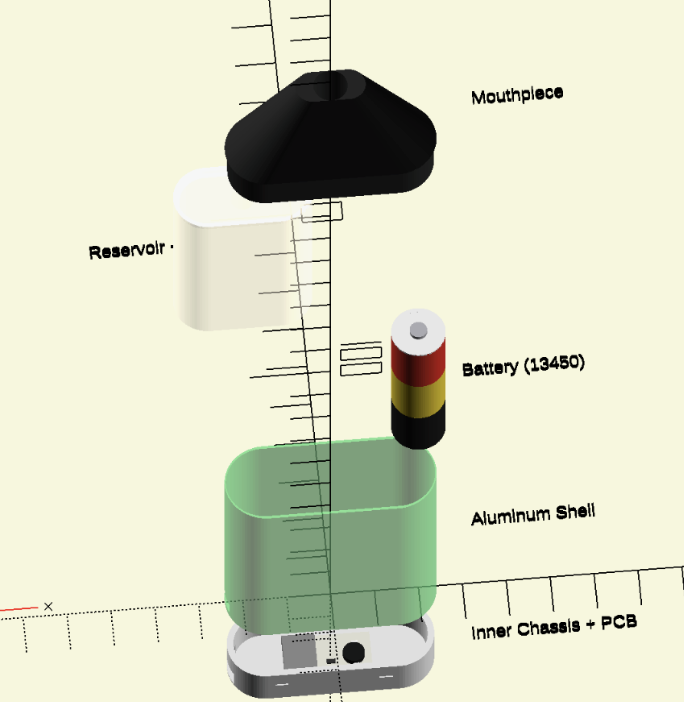
\includegraphics[width=0.4\linewidth]{scad.png}
        \caption{Redesigned Air Bar assembly: exploded view}
    \label{fig:placeholder}
    \end{figure}

\subsection{Device Body Redesign}

Key design changes to the device body:
\begin{enumerate}
    \item \textbf{Housing material}: Switch from aluminum to \textbf{a recycled aluminum alternative} to our impact factor. 
    \item \textbf{Snap-fit assembly}: Two-piece snap-fit inserts that slot into place, and that can be released by pressing down on them. --- no adhesives, no ultrasonic welding, no screws.

    \begin{figure}[H]
        \centering
    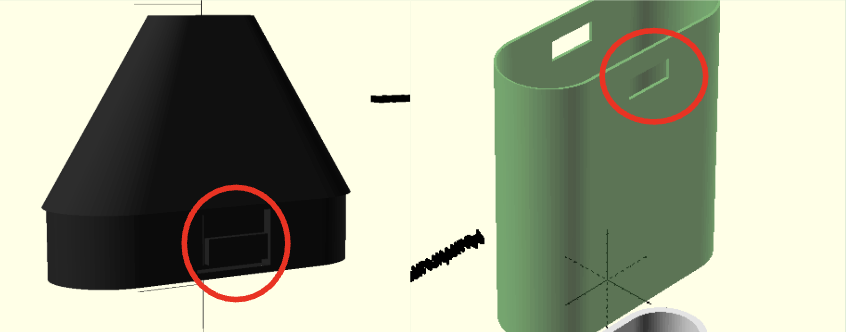
\includegraphics[width=0.7\linewidth]{fit.png}
        \caption{Redesigned snap-fitting assembly}
    \label{fig:placeholder}
    \end{figure}

    \item \textbf{Battery compartment}: Incorporation of quick-disconnect wires would allow the battery to be much more easily swapped, (especially compared to the current hard-wired alternative). 
    \item \textbf{Modular atomizer cartridge}: Slide-in cartridge containing coil, wick, and e-liquid reservoir --- separate recycling stream from battery and housing
    \item \textbf{Standardized PCB mounting}: PCB secured with press-fit standoffs, removable without tools. The same design, but without the need for adhesives. 
\end{enumerate}

\subsection{Impact Reduction Mechanisms}

\begin{enumerate}
    \item \textbf{Battery lifecycle extension}: Each battery reused across 10--450+ device lifecycles instead of 1, reducing per-use lithium demand by 90--99.8\%
    \item \textbf{Elimination of waste stream fires}: Batteries removed before disposal, preventing lithium-ion fires in waste facilities
    \item \textbf{Material recovery}: $>$90\% battery material recovery through established Li-ion recycling pathways (vs.\ $\sim$0\% currently)
    \item \textbf{Reduced raw material extraction}: Less cobalt, nickel, and lithium mining per functional unit
    \item \textbf{Simplified recycling}: Mono-material housing enables single-stream plastic recycling; modular separation eliminates manual sorting
\end{enumerate}

\subsection{LCA of Alternative Concept}

\todo{Run LCA for the alternative concept and present results. Key modeling differences from DfD concept:}
\begin{itemize}
    \item Battery impact allocated across \todo{X} use cycles (not just 1)
    \item Housing material changed from aluminum to PP (lower embodied energy)
    \item End-of-life credits for battery recycling and plastic recycling
    \item Additional: USB-C charging port and spring contacts (marginal)
\end{itemize}

% \begin{figure}[H]
%     \centering
%     \includegraphics[width=0.9\textwidth]{figures/lca_three_way.pdf}
%     \caption{LCA comparison: reference product vs.\ DfD concept vs.\ alternative concept with universal battery standard.}
%     \label{fig:lca_three_way}
% \end{figure}
